%TODO say that you will now prove your claims about the aproach having nearly no impact
%TODO and potentially even claim that you are faster than adevs for some situations, due to the algorithms from PythonPDEVS and further features
%TODO briefly give some hardware info on the machine (CPU, OS, RAM), used software (version of adevs, GCC, ...), and about number of samples/variance
\subsection{Sequential Simulation}
%TODO we start with sequential simulation results, because this is still base case
%TODO compare CPU time with adevs for some benchmarks
%TODO and explain why there is such a difference
%TODO (spend some time here, as this is also important)
%\subsubsection{CPU Usage}
%TODO !!! benchmarks are in integers
The benchmark models are identical in functionality (between adevs/dxex versions). Dxex uses integer timestamps, adevs can only use floating point (of the same values).
\subsubsection{Devstone}
The Devstone \cite{DEVStone} benchmark is highly hierarchical, using Direct connection the dxex kernels can exploit this, whereas adevs needs to walk the structure of the model to pass events.\\
\begin{figure}[h]
	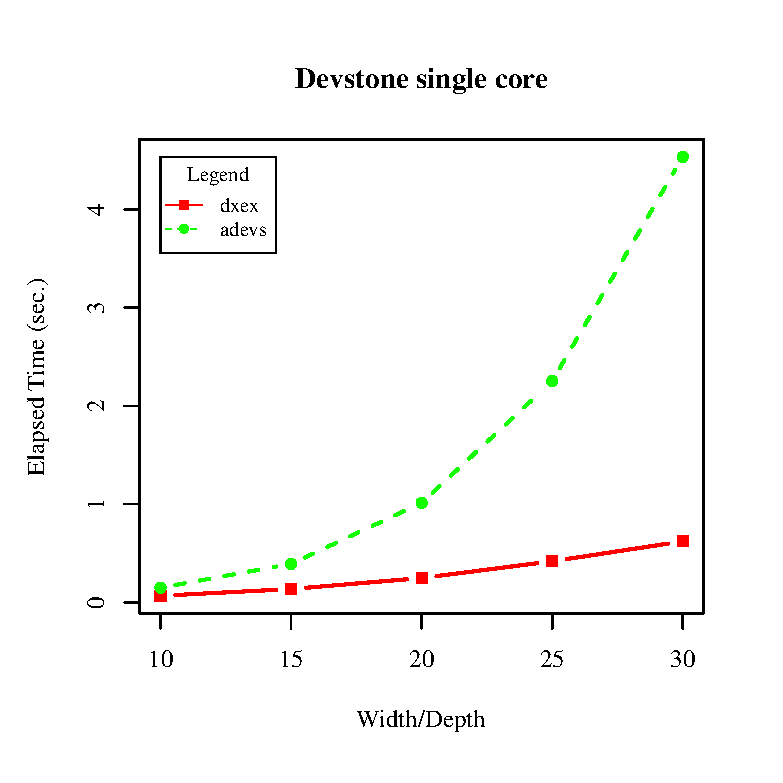
\includegraphics[width=.5\textwidth]{fig/fig1.eps}
	\label{fig1.eps}
\end{figure}

\subsubsection{PHold}
PHold \cite{PHOLD} is a parallel oriented benchmark, sequential runtime is measured only as a baseline. The usage of random nr generators takes up a significant amount of runtime in this model.

\subsubsection{Interconnect}
Interconnect \cite{van2013research} is a benchmark where all models broadcast, creating a complete graph in terms of dependencies between models. As the model count increases, we see the expected quadratic increase in runtime in both kernels, but an increasing penalty for dxex w.r.t. adevs. Profiling shows this is entirely to the heap allocation of the messages by dxex, even though minimized by using memory pools, it remains significant.\\
\begin{figure}[h]
	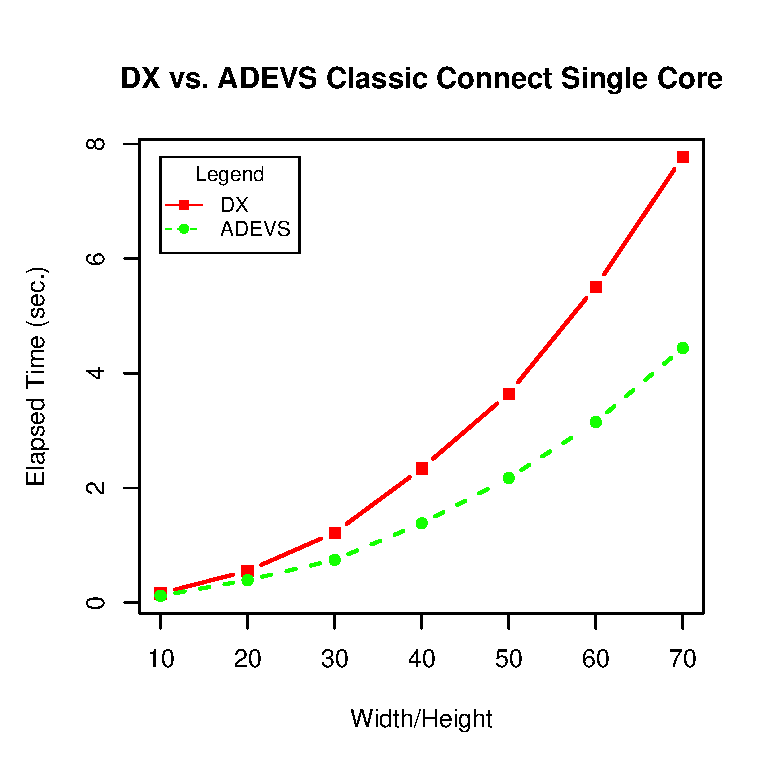
\includegraphics[width=.5\textwidth]{fig/fig3.eps}
	\label{fig3.eps}
\end{figure}

\subsection{Parallel Simulation}
%TODO explain that we will now compare different synchronization protocols
%TODO compare different synchronization protocols with adevs' conservative, showing that we are faster (or at least, not that much slower) than adevs
% split: dstone/pqueue are dag's
\subsubsection{Devstone}
% Initial.
The flattened models are allocated to kernels by giving each kernel a distinct section of the chain, resulting in a low ratio of inter-kernel to intra-kernel messages. For optimistic, this can cause more reverts since the kernels will start to drift faster as the modelcount increases. Furthermore, optimistic is quite sensitive to an increase in kernels, since the delay before a revert propagates increases. Of note as well is the warm-up time this benchmark requires, for $n=d\times w$ models, it takes $\textup{timeadvance}()*n$ transitions to activate the last model in the chain. For parallel this can be reduced to $\frac{ta()*n}{kernels}$ before the last kernel becomes active.\\
\begin{figure}[h]
	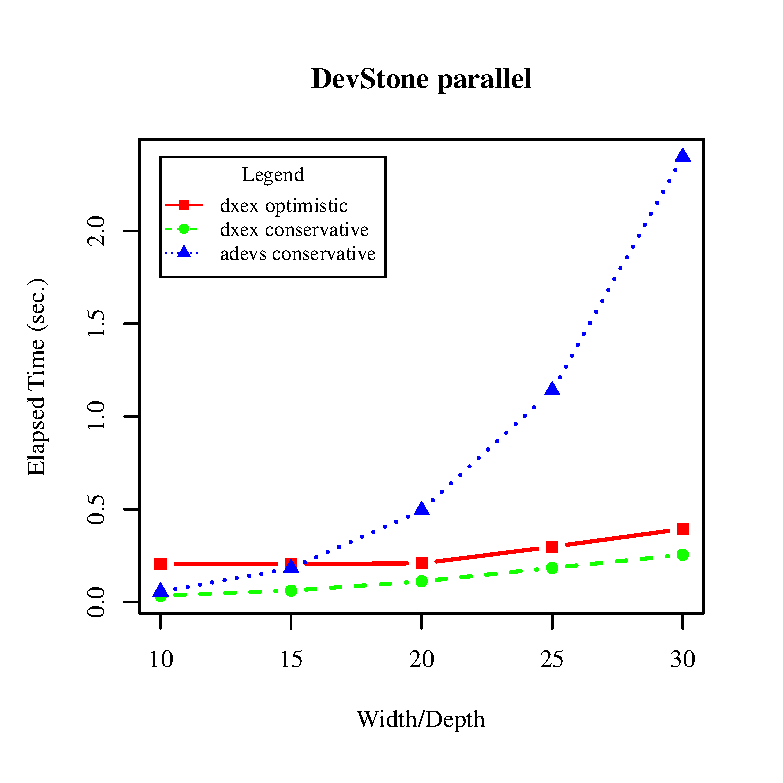
\includegraphics[width=.5\textwidth]{fig/fig2.eps}
	\label{fig2.eps}
\end{figure}
\subsubsection{PHold}
%Phold
In Phold \cite{PHOLD}, allocation is specified in the benchmark itself. Each kernel manages a single node with a constant set of sub-nodes. The parameter R determines the percentage of remote destination models.\\
The dynamic dependency graph is a very sparse version of the static dependency graph, penalizing conservative. Lookahead is $\epsilon$, so conservative spends most of its time crawling in steps of $\epsilon$. Since the dependency graph between kernels is a complete graph, this is not a simulation that scales in our implementation. For N kernels, each kernel has to query the null-time of N-1 kernels, resulting in O($N^2$) polling behaviour. This benchmark therefore highlights the price that we pay for sharing those values instead of sending an actual null message. In a non-cyclic simulation with a non-trivial lookahead (e.g. devstone), that choice however does pay off.\\
Optimistic suffers little from the above problems, however due to the high interconnectivity a cascading revert is still possible. More seriously, a revert is very expensive in PHold due to our usage of C++11's random nr generators. The cost of a revert is dominated by the recalculation of destination models, not in allocating/deallocating states/messages. Again, this could be significantly reduced using lazy-cancellation. Once a revert happens the drift between the kernels increases fast, increasing the likelihood of more reverts. 
\subsubsection{Interconnect}
In Interconnect
the set of atomic models form a complete graph (w.r.t. connections), each model broadcasts messages to the entire set. \\
Allocation is irrelevant, the resulting dependency graph between kernels remains  a complete graph. The runtime dependency graph is almost immediately equal to the static dependency graph.
Conservative still faces the same issues as in PHold, with the key difference that for a fixed time advance lookahead is equal to the timespan between transitions. The scaling issue is identical as in PHold.\\
Our optimistic implementation does not complete an instance of this benchmark. The kernels get stuck in an infinite cascade of reverts. If kernel A reverts, it will send anti-messages to all others who in turn revert and send anti-messages to all others (and A itself again). Support for lazy cancellation could potentially undo this anti-pattern.\\

\subsubsection{Priority network model}
%TODO show a single plot which varies a parameter that changes the ideal synchronization protocol
The priority benchmark is composed of a single server generating a stream of $0<=m<=n$ messages at fixed time intervals, interleaved with a probability p for a priority message, to n receivers. \\ This defaults lookahead for the receivers to $\epsilon$ but this time there is no scaling effect, nor are there cycles in the dependency graph. This model therefore highlights the basic strengths/weaknesses of both synchronization protocols. Receiving models are allocated on another kernel than the server, and have a internal transition so that they will not wait for the incoming messages. 
\input pqueue.tex \\
A key difference here with the other benchmarks is that a state (in the Receiver instances) is very cheap to copy/create. The kernel holding the server will never revert since it is a source in the dependency graph. Optimistic will therefore not suffer the same performance hit in recreating states as it does in PHold. 

%TODO (keep explaining as much as space permits, as this is the evaluation of the core contribution)
\subsection{Memory Usage}
%TODO compare memory usage with adevs for some benchmarks
\subsubsection{Platform and tools}
Both dxex and adevs use tcmalloc as memory allocator. Additionally, dxex uses memory pools to further reduce the frequency of expensive system calls (malloc/free/sbrk/mmap/...). Tcmalloc will only gradually release memory back to the OS, whereas our pools will not do so at all. If memory has been allocated once, it is from a performance point of view better to keep that memory in the pool. For this reason, the memory utilization is best measured by peak allocation. Profiling is done using Valgrind's massif tool \cite{Nethercote:2007:VFH:1273442.1250746}
Platform used has an i5-3317U Intel cpu and 8GB RAM with a page size of 4,096KiB, running Fedora 22 (kernel 4.2.6).\\
\subsubsection{Measure}
Adevs passes messages by value (in container by reference), we pass by pointer. The runtime effects of this choice are already demonstrated in the interconnect benchmark, so in this section, we measure memory usage in number of allocated pages. This combines text, stack and heap memory for the program profiled. From the point of view of the OS or user, this is the actual memory in use. It is important to note that, especially in the case of optimistic, not all this memory is always in use by the kernel. During the simulation, the pools will generally not return memory once allocated, but keep it for later reuse.
\subsubsection{Results}
\paragraph*{Devstone}
\begin{table}[lhtb]
	\centering
	\caption{Devstone 40x40 t5e5, unit MiB, 4 kernels (if parallel)}
	\label{dtone_mem}
	\begin{tabular}{| l | l | l | l | l |}
		\hline
		Adevs & AdevsCon &DX &DXCon &DXOpt\\ \hline
		44 & 70 & 42 & 75 & 363  \\ \hline
	\end{tabular}
\end{table}
Since conservative passes messages by pointer, it needs a GVT/LBTS implementation to organise garbage collection. This inevitable delay explains the higher memory usage compared to adevs.\\
%TODO next sentence needs rewriting --done?
Optimistic needs a more complex GVT/garbage collection algorithm due to the Timewarp algorithm, which requires that the state of models is saved. Additionally, the differences in LP virtual times are far larger compared to conservative time synchronization. All these factors explain the heavier memory usage. Devstone (flattened) is allocated in a chain. The leafs in the dependency graph will therefore do a lot of unnecessary simulation before having a revert, leading to quite severe memory pressure. Unlike conservative and sequential execution, memory usage in optimistic varies greatly depending on scheduling of kernel threads and drifting between kernels. 
\paragraph*{Interconnect}
In section 4.2 the parallel performance of this benchmark is further explained. It is of interest for sequential to contrast with the runtime penalty that dxex suffers w.r.t. adevs. Optimistic fails this benchmark, see section 4.2.3 for a detailed analysis.\\
\begin{table}[lhtb]
	\centering
	\caption{Interconnect w 40 t5e5, unit MiB, 2 kernels (if parallel)}
	\label{iconn_mem}
	\begin{tabular}{| l | l | l | l |}
		\hline
		Adevs & AdevsCon &DX &DXCon\\ \hline
		39 & 39 & 35 & 52  \\ \hline
	\end{tabular}
\end{table}
The discrepancy between both conservative implementations is detailed in 4.1.4.
		
\paragraph*{Priority Network}
The priority network model is detailed in section 4.1.\\
\begin{table}[lhtb]
	\centering
	\caption{Priority model n 16, m 9, p 10,  t5e5, unit MiB, 2 kernels}
	\label{pmod_mem}
	\begin{tabular}{| l | l | l |}
		\hline
		DX &DXCon &DXOpt\\ \hline
		35 & 58 &69\\ \hline
	\end{tabular}
\end{table}
